\subsection{Kavicsos talajon helyben forgás}
A \ref{fig:Left_n50Right50a} megfigyelhető amint a robot kavicsos talajon differenciálisan fordul 60 másodpercen keresztül, ezalatt háromszor teljen korbefordul. A palyat tekintve letrejon egy oldaliranyu mozgás is igy 0.4m kerul odebb. Az oldaliranyu mozgas a nem egyenlo surlodasok es eroeloszlasok miatt jon letre.

\renewcommand{\nth}{2}
\renewcommand{\GlobalPath}{Meresek/Mozgasok/NormalMukodes/DiferencialisanHelybeKavicsos/}
\renewcommand{\secondImage}{*}



\begin{figure}[H]
  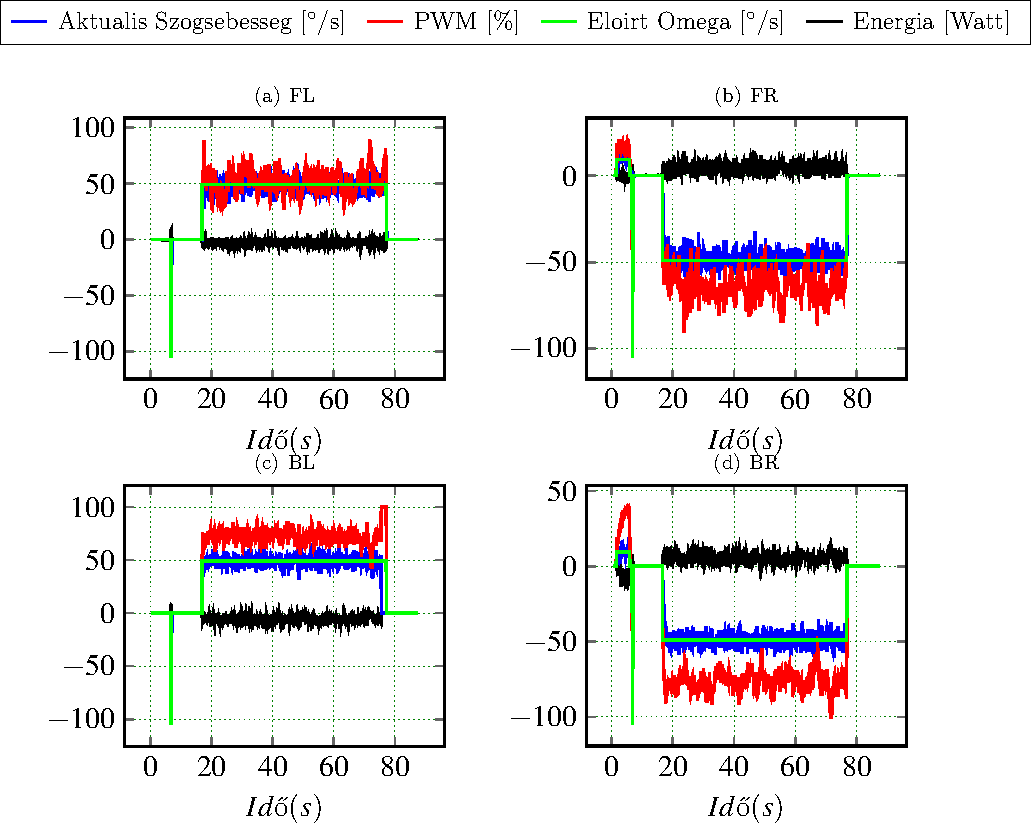
\includegraphics{tikz/Left_n50Right50x.pdf}
  \caption{$SSMR-4W$ típusú robot mozgása, tengelyekre bontva, kereksebessegek BL=FL=0 es a FR=BR= 50\degree/s}
  \label{fig:Left_n50Right50x}
\end{figure}


\begin{figure}[H]
  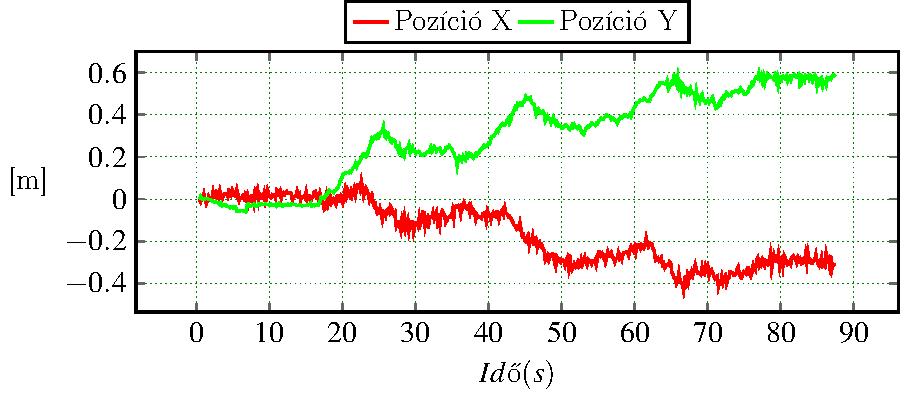
\includegraphics{tikz/Left_n50Right50a.pdf}
  \caption{$SSMR-4W$ típusú robot mozgása, tengelyekre bontva, kereksebessegek BL=FL=-50 es a FR=BR= 50\degree/s}
  \label{fig:Left_n50Right50a}
\end{figure}


\begin{figure}[H]
  \label{fig:Left_n50Right50b}
  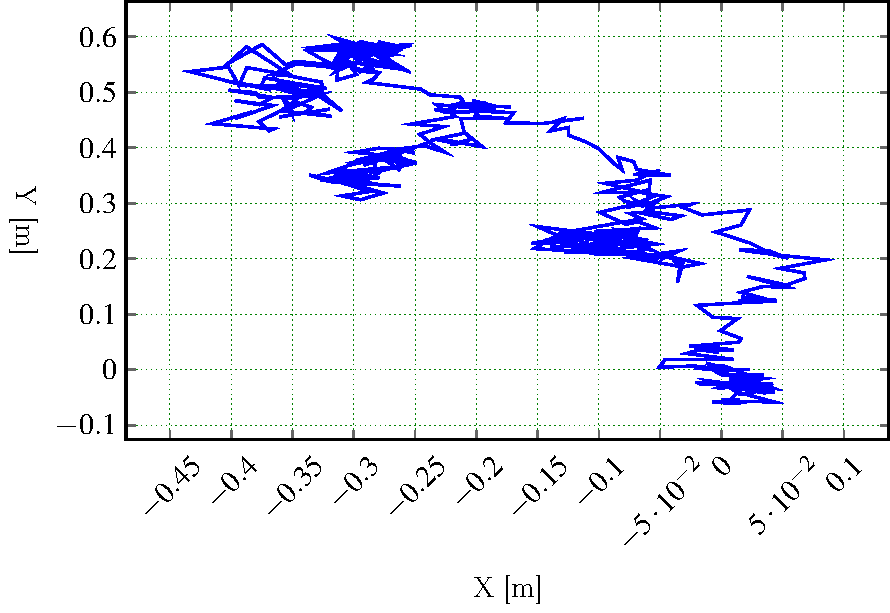
\includegraphics{tikz/Left_n50Right50b.pdf}
  \caption{$SSMR-4W$ típusú robot altal leirt palya, kereksebessegek BL=FL=-50 es a FR=BR= 50\degree/s}
\end{figure}



\begin{figure}[H]
  \label{fig:Left_n50Right50c}
  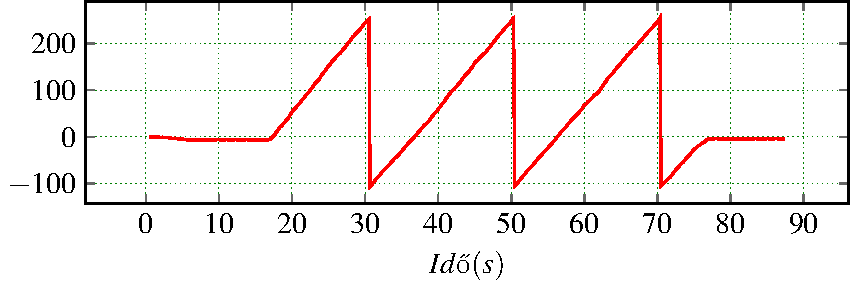
\includegraphics{tikz/Left_n50Right50c.pdf}
  \caption{$SSMR-4W$ típusú robot orientacioja, kereksebessegek BL=FL=-50 es a FR=BR= 50\degree/s}
\end{figure}


\begin{figure}[H]
  \label{fig:Left_n50Right50d}
  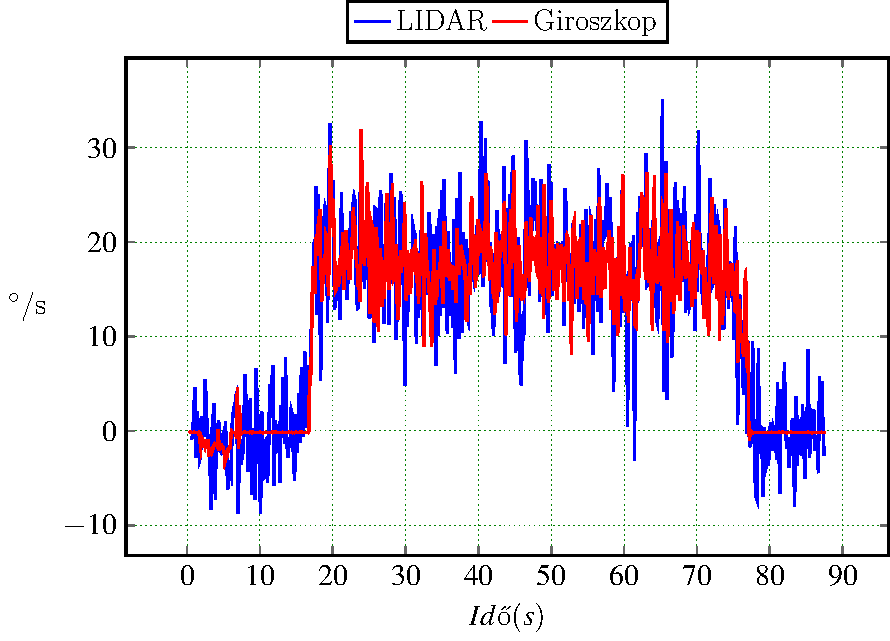
\includegraphics{tikz/Left_n50Right50d.pdf}
  \caption{$SSMR-4W$ típusú robot fordulasi szogsebessege, kereksebessegek BL=FL=-50 es a FR=BR= 50\degree/s}
\end{figure}









